\documentclass[tikz]{standalone}
\usepackage{amsfonts}
\usepackage{amsmath}
\usepackage{amssymb}
\usepackage{tikz}
\begin{document}

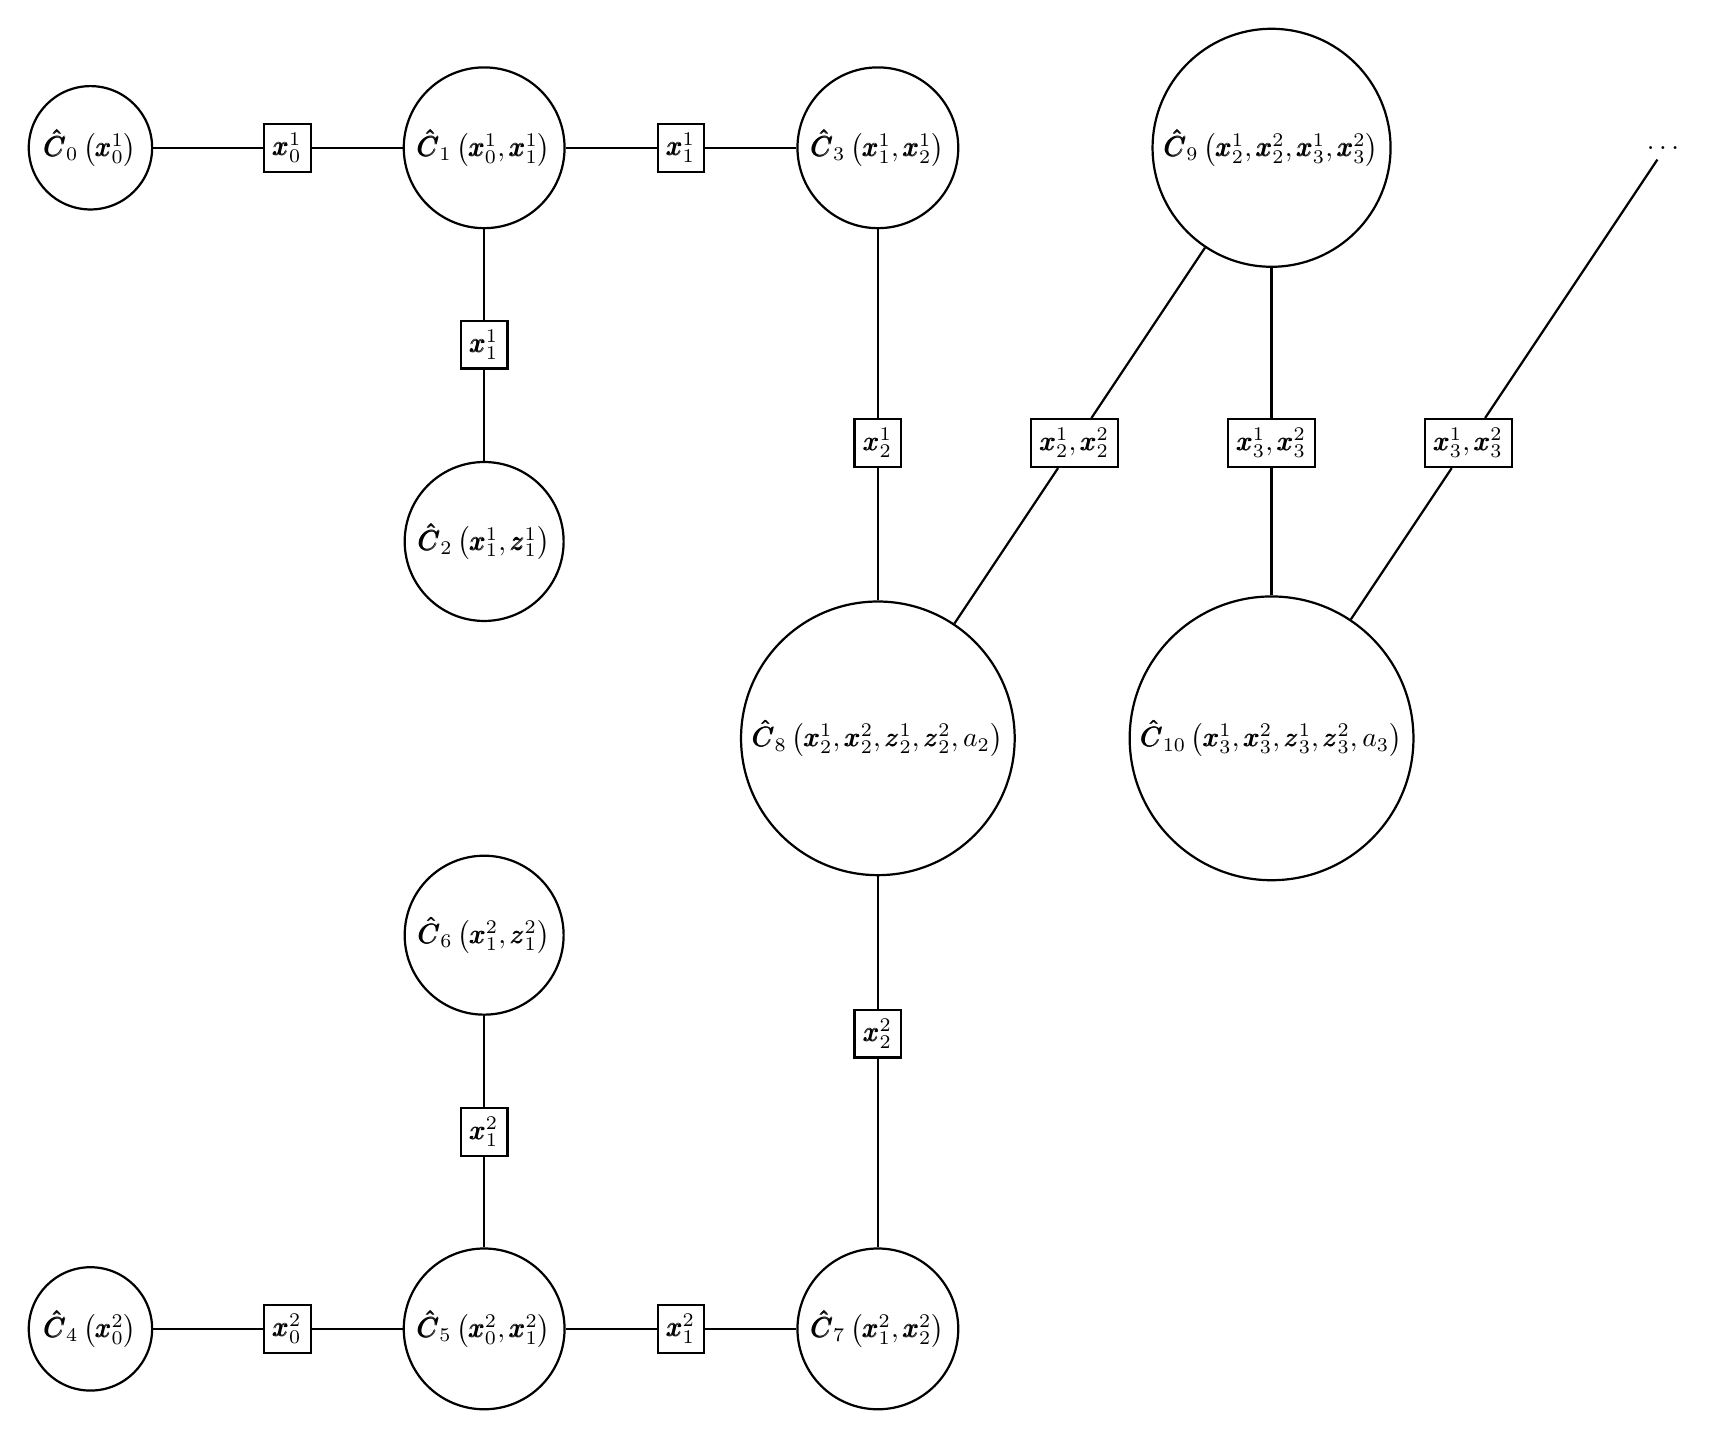
\begin{tikzpicture}
\begin{scope}[every node/.style={circle,thick,draw}]
	%Frame 0
	\node (C_0) at (0, 0) {$\pmb{\hat{C}}_{0} \left( \pmb{x}_{0}^{1} \right)$};
	
	\node (C_4) at (0, -15) {$\pmb{\hat{C}}_{4} \left( \pmb{x}_{0}^{2} \right)$};
	
	%Frame 1
	\node (C_1) at (5, 0) {$\pmb{\hat{C}}_{1} \left( \pmb{x}_{0}^{1}, \pmb{x}_{1}^{1} \right)$};
	\node (C_2) at (5, -5) {$\pmb{\hat{C}}_{2} \left( \pmb{x}_{1}^{1}, \pmb{z}_{1}^{1} \right)$};
	
	\node (C_6) at (5, -10) {$\pmb{\hat{C}}_{6} \left( \pmb{x}_{1}^{2}, \pmb{z}_{1}^{2} \right)$};
	\node (C_5) at (5, -15) {$\pmb{\hat{C}}_{5} \left( \pmb{x}_{0}^{2}, \pmb{x}_{1}^{2} \right)$};
	
	%Frame 2
	\node (C_3) at (10, 0) {$\pmb{\hat{C}}_{3} \left( \pmb{x}_{1}^{1}, \pmb{x}_{2}^{1} \right)$};
	
	\node (C_8) at (10, -7.5) {$\pmb{\hat{C}}_{8} \left(  \pmb{x}_{2}^{1}, \pmb{x}_{2}^{2}, \pmb{z}_{2}^{1}, \pmb{z}_{2}^{2}, a_{2} \right)$};
	
	\node (C_7) at (10, -15) {$\pmb{\hat{C}}_{7} \left( \pmb{x}_{1}^{2}, \pmb{x}_{2}^{2} \right)$};
	
	%Frame 3
	\node (C_9) at (15, 0) {$\pmb{\hat{C}}_{9} \left( \pmb{x}_{2}^{1}, \pmb{x}_{2}^{2}, \pmb{x}_{3}^{1}, \pmb{x}_{3}^{2} \right)$};
	
	\node (C_10) at (15, -7.5) {$\pmb{\hat{C}}_{10} \left(  \pmb{x}_{3}^{1}, \pmb{x}_{3}^{2}, \pmb{z}_{3}^{1}, \pmb{z}_{3}^{2}, a_{3} \right)$};
	
\end{scope}

\begin{scope}[every node/.style={thick,draw}]

	%Frame 0
	\node (s_0^1) at (2.5, 0) {$\pmb{x}_{0}^{1}$};
	
	\node (s_4^5) at (2.5, -15) {$\pmb{x}_{0}^{2}$};
	
	%Frame 1
	\node (s_1^2) at (5, -2.5) {$\pmb{x}_{1}^{1}$};
	\node (s_1^3) at (7.5, 0) {$\pmb{x}_{1}^{1}$};
	
	\node (s_5^6) at (5, -12.5) {$\pmb{x}_{1}^{2}$};
	\node (s_5^7) at (7.5, -15) {$\pmb{x}_{1}^{2}$};
	
	%Frame 2
	\node (s_3^8) at (10, -3.75) {$\pmb{x}_{2}^{1}$};
	
	\node (s_8^9) at (12.5, -3.75) {$\pmb{x}_{2}^{1}, \pmb{x}_{2}^{2}$};	
	
	\node (s_7^8) at (10, -11.25) {$\pmb{x}_{2}^{2}$};
	
	%Frame 3
	\node (s_9^10) at (15, -3.75) {$\pmb{x}_{3}^{1}, \pmb{x}_{3}^{2}$};
	
	\node (s_10^11) at (17.5, -3.75) {$\pmb{x}_{3}^{1}, \pmb{x}_{3}^{2}$};	

\end{scope}

\begin{scope}[style={thick,draw}]
	%Frame 5
    \node (C_11) at (20, 0) {\dots};
\end{scope}

\begin{scope}[style={thick,draw}]

	%Frame 0
	\path [-] (C_0) edge node {} (s_0^1);
	\path [-] (s_0^1) edge node {} (C_1);
	
	\path [-] (C_4) edge node {} (s_4^5);
	\path [-] (s_4^5) edge node {} (C_5);
	
	%Frame 2
	\path [-] (C_1) edge node {} (s_1^2);
	\path [-] (s_1^2) edge node {} (C_2);
	
	\path [-] (C_1) edge node {} (s_1^3);
	\path [-] (s_1^3) edge node {} (C_3);
	
	\path [-] (C_5) edge node {} (s_5^6);
	\path [-] (s_5^6) edge node {} (C_6);
	
	\path [-] (C_5) edge node {} (s_5^7);
	\path [-] (s_5^7) edge node {} (C_7);
	
	%Frame 3
	\path [-] (C_3) edge node {} (s_3^8);
	\path [-] (s_3^8) edge node {} (C_8);
	
	\path [-] (C_8) edge node {} (s_8^9);
	\path [-] (s_8^9) edge node {} (C_9);
	
	\path [-] (C_7) edge node {} (s_7^8);
	\path [-] (s_7^8) edge node {} (C_8);
	
	%Frame 4
	\path [-] (C_9) edge node {} (s_9^10);
	\path [-] (s_9^10) edge node {} (C_10);
	
	\path [-] (C_10) edge node {} (s_10^11);
	\path [-] (s_10^11) edge node {} (C_11);

\end{scope}
\end{tikzpicture}

\end{document}
